\begin{figure*}[t!]
\begin{center}\footnotesize
	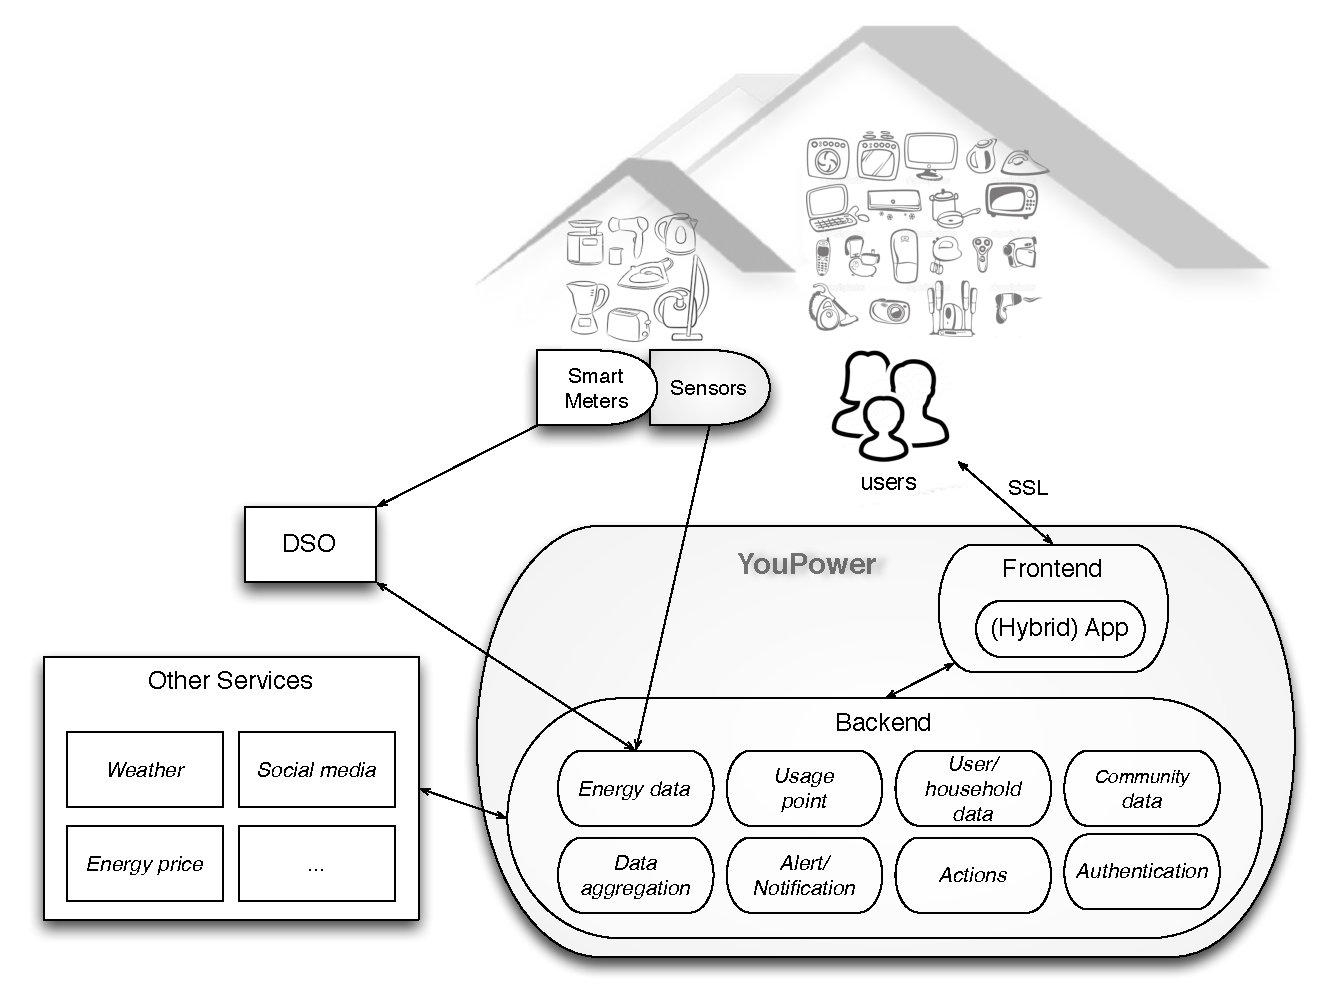
\includegraphics[width=.7\textwidth]{img/civis_platform_overview.pdf}\\
	DSO (Distribution System Operators),  SSL (Secure Sockets Layer)
	\caption{YouPower system overview}\label{fig:platform}
\end{center}
\end{figure*}

\section{\uppercase{State of the Art}}

\noindent Prior to designing YouPower, we review the existing studies with social platforms in the power grid and summarize the lessons learned from those trials. We combine such lessons with the findings from the literature on prosumer behavior change and create a set of design guidelines with successful strategies and potential barriers. A repeatedly reported issue with the solutions aiming to involve prosumers is a lack of long term engagement \cite{edward2015review}. Iterative, open and lean co-design process \cite{folstad2008living,klein2013ux,leffingwell2010agile} that we adopt is suggested as a promising approach to avoid this issue \cite{schwartz2014people}.

\paragraph{Existing social energy platforms.} Weiss et al.~\cite{weiss2012powerpedia} developed a smartphone community platform, PowerPedia. The platform works in connection with smart meters and enables users to identify and upload their own appliance-level consumption statistics. After upload, the users can compare their appliance consumption with other users. The platform was evaluated in a lab setting and the test users rated favorably social comparison features and appliance level statistics. Community Monitor \cite{dillahunt2014understanding} is a social energy app deployed on tablets that was tested in two distinct communities for 4-10 months. The app featured leaderboard, message board and shared actions ("ways to save"). The findings from the trial revealed importance of environmental, social and cultural context for the app use. For instance, the existence of common spaces for community members to interact and knowledge of other users supported the app use. On the other hand, shorter length of residence or rented apartment negatively affected the engagement. Community Monitor did not manage to engage users around the message board feature. Petkov et al.~\cite{petkov2011motivating} delve more into the details of comparative consumption feedback. Their findings confirm the importance of comparison to the similar users and neighbors. However, if the competition features are included, then the users preferred to compete with the people whom they actually know, in particular with friends.
Klimaatstraatfeest\footnote{\url{http://klimaatstraatfeest.nl}} (in Dutch, meaning “climate street party”) is an example initiative by Dutch organization HIER and utility Essent that aims to encourage neighbors (from the same street) to interact with each other and together save energy. In the energy saving competition, the streets compete with each other using online platform through which tips are shared, common actions prepared (such as, buying solar panels) and, based on the activity level, the participants earn points. Gamification is employed in this initiative to encourage both cooperation and competition on a local community level. While in those aspects, similar to the CIVIS platform, Klimaatstraatfeest is focused on local communities and does not allow the users the flexibility to create other type of virtual communities, thus not fully leveraging the potential of ICT.
Opower \cite{allcott2011social}.

\paragraph{Design ideas and guidelines.} The literature review points to several successful interventions for prosumer behavior change. Most of the solutions involve some type of \textit{consumption feedback}, such as individual, historical, real-time, group, and comparative.  YouPower aims to leverage the social aspects, and so we incorporate group (community) feedback because it informs about a collective effort and might enhance the feeling of group efficacy \cite{bandura1997self}. Socially comparative feedback, especially to similar people, has also proven effective \cite{allcott2011social,cialdini2001harnessing,petkov2011motivating}. 


\cite{strengers2011designing} suggests combining feedback with practical recommendations that lead to new practices which challenge taken-for-granted notions of normality. We provide a set of recommended actions.

(2) public commitment: in a commitment making procedure, people are binding to a certain behavior or opinion. In our case, people would make a pledge to perform a certain action to conserve energy. Literature shows that the individuals with a higher need for consistency will be more prone to hold to their commitments (Cialdini, 2001).


(3) modelling: Unlike block leaders, whose influence is used to spread the information in the social network and consequently instigate desired behavior, in role modeling, the models demonstrate the behavior themselves. In this sense, the role models do not need to come from inside the social network, as long as the modelled behavior seems relevant, understandable, rewarding, and meaningful.


(6) the use of social norms in feedback provision: difference to the socially comparative feedback, a similar type of measure, is that the use of social norms means that the standards and rules are established about the behavior for the members of some group. The social norms are about what other people approve or disapprove doing. According to (Cialdini et al., 1991), when made salient, such norms guide behaviour.


X Considering the analytical frames and the CIVIS use cases, we chose a set of platform features and translated those into three self-contained and composable parts to be included in the CIVIS (front-end) application (hereinafter abbreviated as CIVIS app): 
%\begin{enumerate}
%\item \nameref{sect:tips}
%\item \nameref{sect:brf}
%\item \nameref{sect:load_shifting}
%\end{enumerate}



With peer review results and users' feedback on the design, adaptations and changes are made to suit user needs and to achieve the CIVIS research goal. 
In general, the application aims to enhance users' energy know-how through action suggestions that are implementable in everyday life, engage users in energy communities with understandable and actionable information and feedback, and facilitate community interaction and self-teaching by means of group discussions.
%

Given the time and resource constraints, the app can not be developed all-in-one cross-platform (for phones, tablets and computers). We chose to design the front-end as a mobile app. This means that the app design has layouts and user interactions that suit (small) phone screens. %The consideration is multi-fold. 
Western Europe has a large mobile phone internet user base\footnote{
Between 2013 and 2017, the penetration rate of mobile phone internet users among mobile phone users will rise from 49.0\% to 77.8\%. See more at: \url{ http://www.emarketer.com/Article/Nearly-Half-of-Western-Europeans-Will-Use-Mobile-Web-This-Year/1010510\#sthash.AaVfsqIU.dpuf}}. Many surveys show that mobile apps have advantages such as creating deeper user engagement, easy sharing, among others\footnote{\url{https://infomedia.com/blog/the-advantages-of-mobile-apps/}, \url{https://econsultancy.com/blog/62326-85-of-consumers-favour-apps-over-mobile-websites/}}. This makes mobile app a good choice given the goal of the CIVIS platform. Once developed, mobile apps can also be more easily transformed to web browser versions, while the reverse is more difficult. The back-end of the CIVIS platform will remain mostly the same independent of the front-end alternatives. 